\chapter{How to install LELAPE}
\section{Why Julia?}
The Julia language (\href{https://julialang.org}{https://julialang.org}] was released in 2012 as a possible solution the classical \textit{``Two Languages' Problem"}: a language easy to learn and develop in is usually slow and vice versa, so too often algorithms must be developed in one language and rewritten in another more efficient one (Fig. \ref{Fig:Shah_trolling_Elon}). This language was specifically built to achieve speed, efficiency and clarity  \cite{bezanson2017julia}.
%
\begin{figure}
	\centering
	
\includegraphics[width=0.5\textwidth]{fig/Shah_and_musk.png}
	\caption{An example of not using Julia and working twice  (\href{https://twitter.com/Viral_B_Shah/status/1224362465779163138}{https://twitter.com/Viral \_B\_Shah/status/1224362465779163138})}.
	\label{Fig:Shah_trolling_Elon}
\end{figure}

\section{How to install Julia}
%
Julia, open software released with MIT license, can be downloaded and installed from
\begin{center}
 \href{https://julialang.org/downloads/}{https://julialang.org/downloads/} 
\end{center}
for different operating systems and architectures. Depending on the system, the binary files will be installed (Microsoft Windows, macOS) or just uncompressed (GNU/Linux, FreeBSD). Compilation from source code is also possible.

\begin{figure}
	\centering
	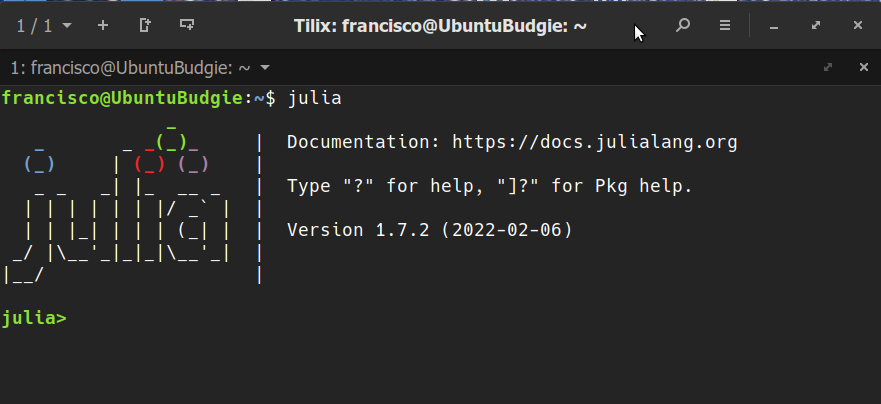
\includegraphics[width=0.65\textwidth]{fig/Julia_REPL} 
	\\(a)\\
	\vspace{1cm}
	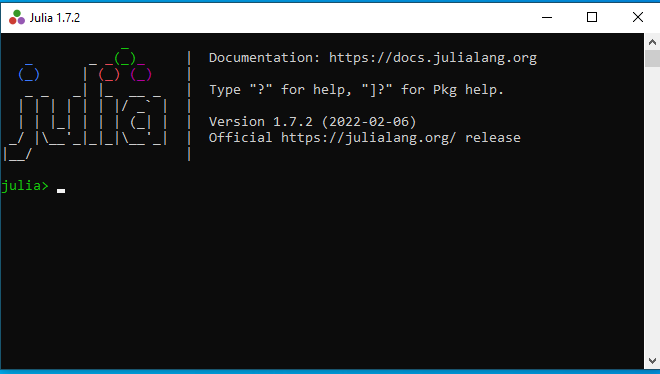
\includegraphics[width=0.65\textwidth]{fig/julia_in_windows}
	\\(b)\\
	\caption{Example of the REPL's welcome screen for Julia on a machine running Ubuntu Budgie (a) and Microsoft Windows (b).}
	\label{Fig;JuliaREPL}
\end{figure}
%
If no additional tool is installed, Julia will be executed in a REPL as it is shown in Fig. \ref{Fig;JuliaREPL}. However, most of the users prefer to use the language in conjunction with Integrated Development Environments (IDE) or notebooks such as:`

\begin{itemize}
	\item \textbf{Visual Studio Code}: Popular IDE developed by Microsoft with plugins for Julia. It can be downloaded from \href{https://code.visualstudio.com/}{https://code.visualstudio.com/} and the plugins installed as extensions. See \href{https://code.visualstudio.com/docs/languages/julia}{https://code.visualstudio.com/docs/languages/julia} for further information.
	%
	\item \textbf{Jupyter}: Although it is typically used for Python, it is also appropriate for Julia. Indeed, Jupyter is an acronym for \textbf{Ju}lia-\textbf{Pyt}hon-\textbf{R}. There are different ways of installing Jupyter. In systems with Microsoft Windows OS, the most simple way is to install Anaconda (\href{https://www.anaconda.com/products/individual}{https://www.anaconda.com/products/individual}). It can be setup to use Julia as calculation engine. In GNU/Linux there are smaller packages to install Jupyter. For example, in Ubuntu the simple instruction \texttt{sudo apt install jupyter-notebook} will install the software in your computer. Later, it is necessary to install an additional package inside Julia but this will be studied a bit later.
	
	Modern versions of Julia allow skipping this step, as we will see later. If Jupyter is not found, Julia  downloads and locally installs the software.
	%
	\item \textbf{Pluto}: A notebook following the philosophy of Jupyter but specifically developed for Julia and easily extensible with JavaScript. Unlike the previous tools, it is installed inside Julia, not along with it. 
\end{itemize}
%
Jupyter and Pluto require the installation of additional packages to link Julia to the IDE. As Jupyter is probably the most popular tool, it is installed inside Julia REPL with the following instructions:

\vspace{1mm}
\begin{center}
	\texttt{using Pkg; Pkg.add("IJulia")}
\end{center}
\vspace{1mm}

This adds the package IJulia to the basic Julia installation. However, a previous step is to search for Jupyter on your computer. In the case of not finding it, Julia suggests to download a minimal version of Conda, thus installing Jupyter, as shown in Fig. \ref{Fig:Installling_Conda_with_julia}. Finally, it is launched  inside Julia as follows:
%
\begin{figure}
	\centering
	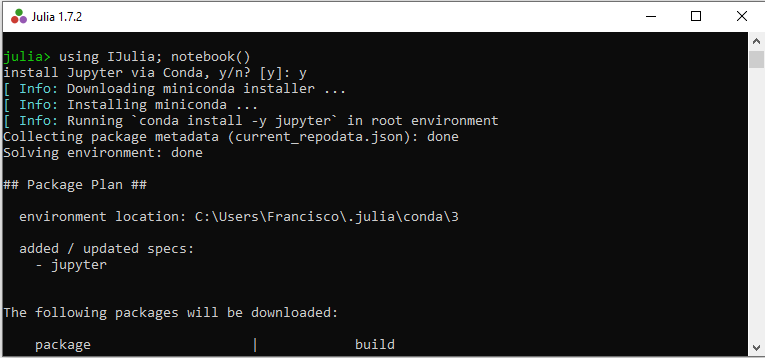
\includegraphics[width=0.65\textwidth]{fig/Julia_using_miniconda}
	\caption{If Jupyter is not detected, Julia installs a minimal version the first time IJulia is used.}
	\label{Fig:Installling_Conda_with_julia}
\end{figure}

\vspace{1mm}
	\begin{center}
		\texttt{using IJulia; notebook()} 
	\end{center}
\vspace{1mm}

Pluto package is installed following a similar procedure. 

\vspace{1mm}
\begin{center}
	\texttt{using Pkg; Pkg.add("Pluto");}
\end{center}
\vspace{1mm}

and launched with:

\vspace{1mm}
\begin{center}
	\texttt{using Pluto; Pluto.run()}
\end{center}
\vspace{1mm}

There are other options if you prefer cloud computing. For  example, in spite of the fact that its primary use is running Python code, Google Colab is compatible with Julia language. For further information (and also learning a little Julia), you can read \href{https://colab.research.google.com/github/ageron/julia_notebooks/blob/master/Julia_for_Pythonistas.ipynb#scrollTo=GIeFXS0F0zww}{Julia for Pythonists} and use the \href{https://colab.research.google.com/github/ageron/julia_notebooks/blob/master/Julia_Colab_Notebook_Template.ipynb}{Julia Colab Template}. However, this solution is not recommended due to some problems at installing external packages as well as at loading data files. Perhaps this flaw can be fixed in the future, but, nowadays, the tool is not as powerful as the others.

\section{Installing LELAPE}
%
LELAPE is built as a module. In Julia, a module is a set of elements such as variables, functions, etc. that can be loaded at will. The procedure is the following:
%
\begin{enumerate}
	\item Download the ZIP system from \href{https://zenodo.org/records/10156119}{Zenodo} and decompress it. Alternatively, you can clone the site with \texttt{git}. The instruction is \\ \texttt{git clone https://github.com/fjfrancopelaez/LELAPE.git}
	%
	\item Find the \texttt{LELAPE/src} folder where a file called LELAPE.jl is located.
	%
	\item Copy the full path pointing to this folder (\texttt{PATH\_TO\_FOLDER}) and execute in REPL, Jupyter or the notebook you use the following command:
	
	\vspace{1mm}
	\begin{center}
		\texttt{{push!(LOAD\_PATH,"PATH\_TO\_FOLDER")}}
	\end{center}
	\vspace{1mm}	
	
	For example, if LELAPE.jl is found in \texttt{/home/johndoe/Download/LELAPE/src/}, the instruction is:
		
	\vspace{1mm}
	\begin{center}
		\texttt{push!(LOAD\_PATH, "/home/johndoe/Download/LELAPE/src")}
	\end{center}
	\vspace{1mm}	
	
	Thus, Julia knows where to find the module. \texttt{LOAD\_PATH} is a string vector that contains the list of folder where Julia must look up external libraries. \texttt{push!} is a function that adds a new element at the end of any vector, keeping the name. Therefore, we have just added a new entry to the original list.	Fig. \ref{Fig:Loading_LELAPE} is a snapshot of the Julia terminal in GNU/Linux.
	%
	\begin{figure}
		\centering
		
		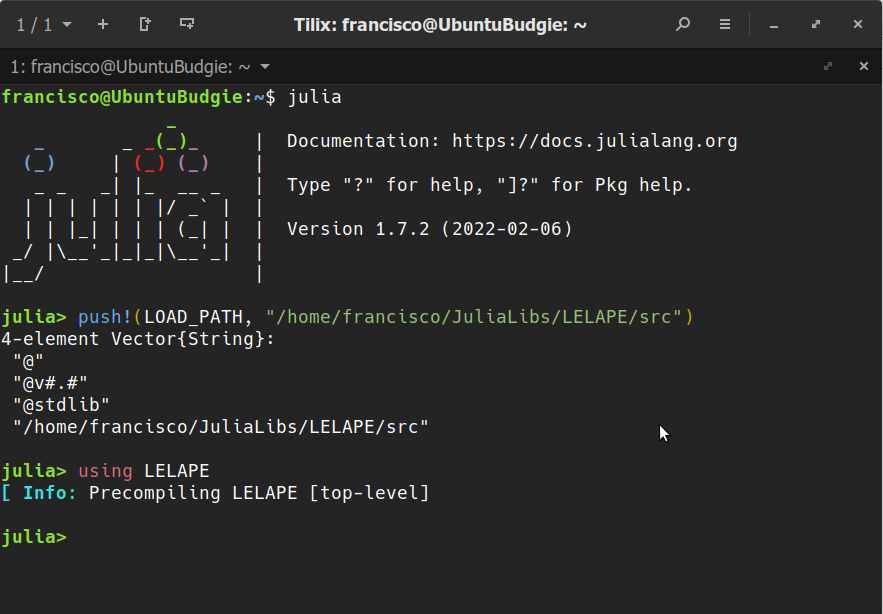
\includegraphics[width=0.65\textwidth]{fig/Loading_LELAP.png}
		\caption{How to indicate Julia where LELAPE is installed, and how to load it.}
		\label{Fig:Loading_LELAPE}
	\end{figure}
	
	A warning for users of Microsoft Windows: in this operating system, folders in the path are marked with the symbol \texttt{$\backslash$}. For technical reasons, this is not recognized by Julia, so the path to LELAPE must be modified with one of the following tips:
	%
	\begin{itemize}
		\item Replacing  \texttt{$\backslash$} with \texttt{/}, emulating the Unix style (GNU/Linux and Mac OS X).
		\item Replacing \texttt{$\backslash$} with \texttt{$\backslash\backslash$}.
	\end{itemize}
	%
	Fig. \ref{Fig:LELAPE_PATH_Windows} shows how to sucessfully add a new element to \texttt{LOAD\_PATH} with the first option\footnote{The instruction was \texttt{push!(LOAD\_PATH, "C:/Users/francisco/Desktop/LELAPE-main/LELAPE/src")}, although \texttt{push!(LOAD\_PATH, "C:{\textbackslash\textbackslash}Users{\textbackslash\textbackslash}francisco{\textbackslash\textbackslash}Desktop{\textbackslash\textbackslash}LELAPE-main{\textbackslash\textbackslash}LELAPE {\textbackslash\textbackslash}src")}}.
	%
	\begin{figure}
		\centering
		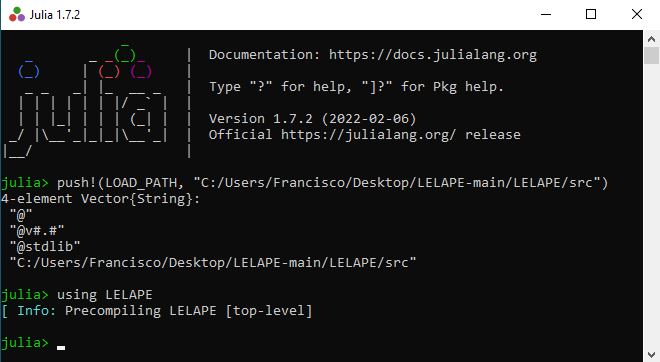
\includegraphics[width=0.65\textwidth]{fig/Julia_loading_LELAPE}
		\caption{The folder containing LELAPE is added to the admitted paths in Microsoft Windows.}
		\label{Fig:LELAPE_PATH_Windows}
	\end{figure} 

	\item Now, just launch LELAPE with the following instruction:
		
	\vspace{1mm}
	\begin{center}
		\texttt{using LELAPE}
	\end{center}
	\vspace{1mm}	
		
	After a few seconds to precompile the library, the functions are loaded. Figs. \ref{Fig:Loading_LELAPE}--\ref{Fig:Julia_in_macos} show practical examples.
\end{enumerate}

\begin{figure}
	\centering
	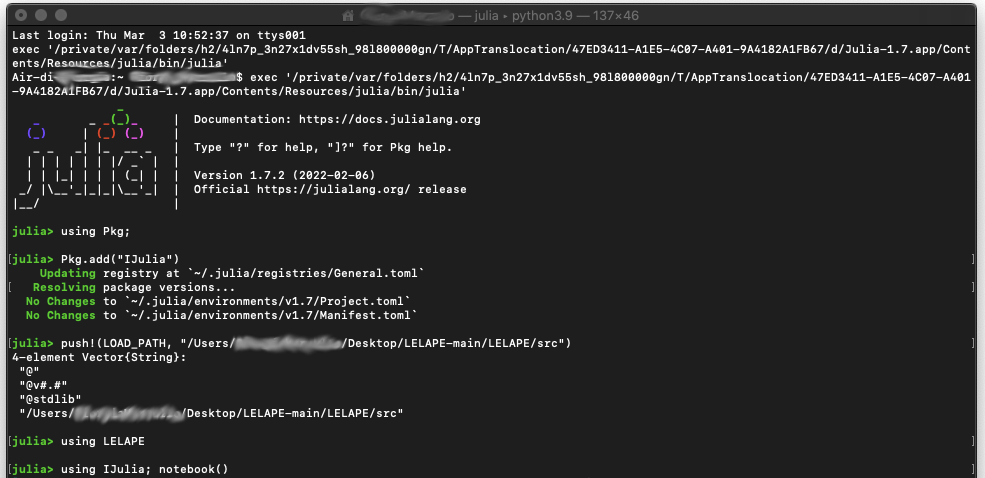
\includegraphics[width=0.65\textwidth]{fig/Julia_in_macOS_anonymous}
	\caption{Executing Julia on macOS and loading LELAPE.}
	\label{Fig:Julia_in_macos}
\end{figure}

Jupyter users should be aware of a detail. Even if it is loaded on the terminal, it does not inherit loaded packages or modules, so they must be loaded again and independently in Jupyter. Even more, the \texttt{LOAD\_PATH} variable is initialized with its default value, with only three elements, so the instruction \texttt{push!(LOAD\_PATH, "PATH\_TO\_FOLDER")} must be executed again before loading LELAPE.

\section{Recommended packages}
%
There are many Julia packages at the user's disposal that can be found on

\begin{center}
	\href{https://juliapackages.com/}{https://juliapackages.com/}.
\end{center}  

Some packages are extremely popular:
\begin{itemize}
	\item \textbf{Revise}: Useful for code developers since it allows reloading user functions without restarting Julia and losing information.
	\item \textbf{OhMyREPL}: Inteligent highlighting of elements in REPL. Figs. \ref{Fig;JuliaREPL} \& \ref{Fig:Loading_LELAPE} are using this package to show function names and strings.
\end{itemize}

Both are installed with \texttt{Pkg.add()}. \vspace{5mm}

Also the package \textbf{Printf} is recommended, since it is used by some scripts in the example section. The macro \textbf{{\makeatletter @}printf} allows printing information on the screen following the C convention.

Another interesting package to have is \textbf{DelimitedFiles}, which allows reading and writing CSV files. It is an essential package in Julia, available in a fresh installation, but not loaded by default. It is not necessary to fetch it and it is loaded as:
	
\vspace{1mm}
\begin{center}
	\texttt{using DelimitedFiles}
\end{center}
\vspace{1mm}	

This package is necessary to use the illustrative Jupyter notebooks that are provided along with LELAPE.

\textbf{A tip for new users}: after working with Julia for a long time, you may eventually discover that only a few packages are frequently used and  you may get bored of loading them every time you start a new session. Thus, the typical solution is to create the following folder and text file in your home directory:
%
\begin{itemize}
	\item In GNU/Linux \& Mac OS X: \texttt{/home/<USER>/.julia/config/startup.jl}
	\item In Microsoft Windows: \texttt{C:{\textbackslash}Users{\textbackslash}<USER>{\textbackslash}.julia{\textbackslash}config{\textbackslash}startup.jl}
\end{itemize}  
%
Fig. \ref{Fig:startup.jl} is an example of the \texttt{startup.jl}. In this file, one can see that LELAPE placement is automatically loaded when the session begins. However, if you wish to load these packages in Jupyter, it is necessary to create a new file, \texttt{startup\_ijulia.jl}, with identical information. However, a soft link to \texttt{startup.jl} is enough.
%
\begin{figure}
	\centering
	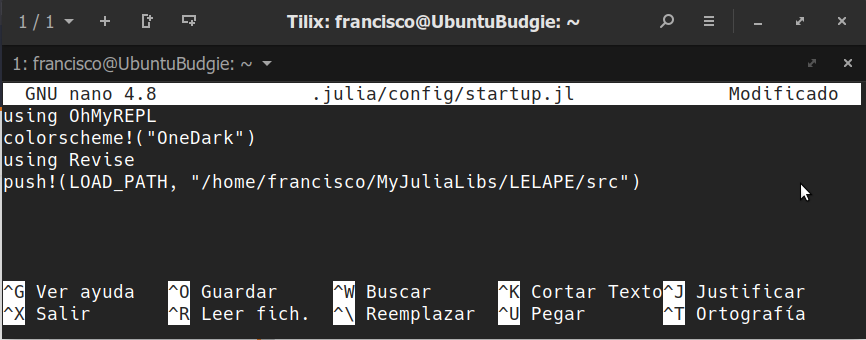
\includegraphics[width=0.65\textwidth]{fig/startup.jl}
	\caption{Example of \texttt{startup.jl} file in GNU/Linux.}
	\label{Fig:startup.jl}
\end{figure} 